\makeatletter
\makeatother

% \documentclass[whitelogo, roman, parspace, oneside, draft]{tudelft-report}
\documentclass[whitelogo, roman, parspace, oneside]{tudelft-report}


\usepackage{csquotes}
\usepackage[style=apa]{biblatex}
\addbibresource{report/bibliography/zotero_bib.bib}

\usepackage[todonotes={color=green!40}]{changes}
\usepackage{comment}

\makenomenclature
\begin{document}


\newcommand{\partdiff}[2]{\frac{\partial #1}{\partial #2}}
\newcommand{\partdifff}[2]{\frac{\partial^2 #1}{\partial #2^2}}
\newcommand{\diff}[2]{\frac{d #1}{d #2}}
\newcommand{\difff}[2]{\frac{d^2 #1}{d #2^2}}

%% Use Roman numerals for the page numbers of the title pages and table of
%% contents.
\frontmatter

%% Uncomment following 19 lines for a cover with a picture on the lower half only
\title[tudelft-white]{Literature review}
\subtitle[tudelft-black]{Efficient modelling of time-domain dynamic positioning simulations}
\author[tudelft-white]{A.W.N. Aperghis}
\affiliation{Technische Universiteit Delft}
\coverimage{report/images/cover/Rosmari_Allseas Solitaire_Drone_15.jpg}
\titleoffsetx{1cm}
\titleoffsety{10cm}
\afiloffsetx{1cm}
\afiloffsety{18cm}
\covertext[tudelft-white]{
}
\setpagecolor{tudelft-cyan}
\makecover[whitelogo]


%% Include an optional title page.
% \input{title}
% Define groups and their names for nomentbl style (tabular)
\renewcommand{\nomgroup}[1]{%
\ifthenelse{\equal{#1}{A}}{\item[\textbf{Acronyms}]}{%
\ifthenelse{\equal{#1}{M}}{\item[\textbf{Mathematical Symbols}]}{%
\ifthenelse{\equal{#1}{O}}{\item[\textbf{Operators and Functions}]}{}}}}

% Nomenclature format: \nomenclature[Group]{Symbol}{Description}{Units}{Note}
% Note: Units are automatically wrapped in \si{} command by nomentbl package
\nomenclature[A]{ASOG}{Activity Specific Operating Guideline}{}{}
\nomenclature[A]{BNN}{Bayesian Neural Network}{}{}
\nomenclature[A]{CPU}{Central Processing Unit}{}{}
\nomenclature[A]{DMD}{Dynamic Mode Decomposition}{}{}
\nomenclature[A]{DP}{Dynamic Positioning}{}{}
\nomenclature[A]{DPO}{Dynamic Positioning Operator}{}{}
\nomenclature[A]{eDMD}{Extended Dynamic Mode Decomposition}{}{}
\nomenclature[A]{GELU}{Gaussian Error Linear Unit}{}{}
\nomenclature[A]{gPC}{Generalized Polynomial Chaos}{}{}
\nomenclature[A]{GPU}{Graphics Processing Unit}{}{}
\nomenclature[A]{GRU}{Gated Recurrent Unit}{}{}
\nomenclature[A]{IMCA}{International Marine Contractors Association}{}{}
\nomenclature[A]{KL}{Kullback--Leibler}{}{}
\nomenclature[A]{MARIN}{Maritime Research Institute Netherlands}{}{}
\nomenclature[A]{MC}{Monte Carlo}{}{}
\nomenclature[A]{MCMC}{Markov Chain Monte Carlo}{}{}
\nomenclature[A]{MIONet}{Multiple-Input Operator Network}{}{}
\nomenclature[A]{NARX}{Nonlinear Auto-Regressive with eXogenous input}{}{}
\nomenclature[A]{NED}{North-East-Down}{}{}
\nomenclature[A]{OU}{Ornstein-Uhlenbeck}{}{}
\nomenclature[A]{PCE}{Polynomial Chaos Expansion}{}{}
\nomenclature[A]{PID}{Proportional-Integral-Derivative}{}{}
\nomenclature[A]{RAM}{Random Access Memory}{}{}
\nomenclature[A]{SDE}{Stochastic Differential Equation}{}{}
\nomenclature[A]{SDE-GAN}{Stochastic Differential Equation Generative Adversarial Network}{}{}
\nomenclature[A]{TD-gPC}{Time-Dependent Generalized Polynomial Chaos}{}{}
\nomenclature[A]{UQ}{Uncertainty Quantification}{}{}
\nomenclature[A]{VI}{Variational Inference}{}{}
\nomenclature[A]{VAMP}{Variational Approach for Markov Processes}{}{}
\nomenclature[A]{VRAM}{Video Random Access Memory}{}{}


\nomenclature[M]{$\eta$}{Position vector in NED frame}{\meter, \radian}{}
\nomenclature[M]{$\dot{\eta}$}{Time derivative of position vector}{\meter\per\second, \radian\per\second}{}
\nomenclature[M]{$\nu$}{Body-fixed velocity vector}{\meter\per\second, \radian\per\second}{}
\nomenclature[M]{$\dot{\nu}$}{Time derivative of velocity vector}{\meter\per\second\squared, \radian\per\second\squared}{}
\nomenclature[M]{$J(\eta)$}{Rotation matrix from body-fixed to NED frame}{-}{}
\nomenclature[M]{$\eta_d$}{Desired position and heading setpoint}{\meter, \radian}{}
\nomenclature[M]{$\hat{\eta}$}{Estimated position from state observer}{\meter, \radian}{}
\nomenclature[M]{$\tilde{\eta}$}{Position error ($\hat{\eta} - \eta_d$)}{\meter, \radian}{}
\nomenclature[M]{$\tilde{\dot{\eta}}$}{Velocity error (time derivative of error)}{\meter\per\second, \radian\per\second}{}
\nomenclature[M]{$\tau$}{Generalized external force vector}{\newton, \newton\meter}{}
\nomenclature[M]{$\tau_{PID}$}{PID controller output force and torque vector}{\newton, \newton\meter}{}
\nomenclature[M]{$\tau_{wind}$}{Wind force and torque in body-fixed frame}{\newton, \newton\meter}{}
\nomenclature[M]{$K_{ff}$}{Feed-forward gain for wind compensation}{-}{}
\nomenclature[M]{$M_{RB}$}{Rigid-body mass matrix}{\kilogram}{}
\nomenclature[M]{$M_A$}{Hydrodynamic added-mass matrix}{\kilogram}{}
\nomenclature[M]{$C_{RB}(\nu)$}{Rigid-body Coriolis-centripetal matrix}{\kilogram\per\second}{}
\nomenclature[M]{$C_A(\nu)$}{Added-mass Coriolis-centripetal matrix}{\kilogram\per\second}{}
\nomenclature[M]{$D$}{Linear damping matrix}{\kilogram\per\second}{}
\nomenclature[M]{$D_n(\nu)$}{Nonlinear damping matrix}{\kilogram\per\second}{}
\nomenclature[M]{$G$}{Restoring matrix}{\newton\per\meter, \newton\meter\per\radian}{}
\nomenclature[M]{$H_s$}{Significant wave height}{\meter}{}
\nomenclature[M]{$T_p$}{Peak wave period}{\second}{}
\nomenclature[M]{$S(\omega)$}{Wave spectral density as function of frequency}{\meter\squared\per\radian\per\second}{}
\nomenclature[M]{$N$}{Total number of wave components in spectral decomposition}{-}{}
\nomenclature[M]{$A_j$}{Amplitude of wave component $j$}{\meter}{}
\nomenclature[M]{$\omega_j$}{Angular frequency of wave component $j$}{\radian\per\second}{}
\nomenclature[M]{$k_{x,j}$}{X-direction wave number for component $j$}{\radian\per\meter}{}
\nomenclature[M]{$k_{y,j}$}{Y-direction wave number for component $j$}{\radian\per\meter}{}
\nomenclature[M]{$\epsilon_j$}{Random phase angle for wave component $j$}{\radian}{}
\nomenclature[M]{$\Delta\omega$}{Frequency spacing or bandwidth increment}{\radian\per\second}{}
\nomenclature[M]{$V_w$}{Wind speed}{\meter\per\second}{}
\nomenclature[M]{$\mathbf{u}(t)$}{Input signal/vector to dynamical system}{Varies}{}
\nomenclature[M]{$\mathbf{y}(t)$}{Output/measurement vector from system}{Varies}{}
\nomenclature[M]{$A$}{State transition matrix (continuous-time SSM)}{-}{}
\nomenclature[M]{$B$}{Input matrix (continuous-time SSM)}{-}{}
\nomenclature[M]{$C$}{Output/measurement matrix (continuous-time SSM)}{-}{}
\nomenclature[M]{$\bar{A}$}{Discrete-time state transition matrix}{-}{}
\nomenclature[M]{$\bar{B}$}{Discrete-time input matrix}{-}{}
\nomenclature[M]{$\bar{C}$}{Discrete-time output/measurement matrix}{-}{}
\nomenclature[M]{$\mathbf{f}(\cdot)$}{Continuous-time dynamics function}{-}{}
\nomenclature[M]{$\mathbf{F}(\cdot)$}{Discrete-time dynamics map}{-}{}
\nomenclature[M]{$\boldsymbol{\beta}$}{Model parameter vector}{Varies}{}
\nomenclature[M]{$x$}{Model input variable}{Varies}{}
\nomenclature[M]{$y$}{Model output variable}{Varies}{}
\nomenclature[M]{$f(\cdot)$}{Model mapping inputs to outputs}{-}{}
\nomenclature[M]{$X$}{Random variable}{Varies}{}
\nomenclature[M]{$\omega$}{Elementary event in $\Omega$}{-}{}
\nomenclature[M]{$\Omega$}{Sample space}{-}{}
\nomenclature[M]{$\mathcal{F}$}{Sigma-algebra}{-}{}
\nomenclature[M]{$\mathbb{P}$}{Probability measure}{-}{}
\nomenclature[M]{$\boldsymbol{\xi}$}{Vector of random variables}{Varies}{}
\nomenclature[M]{$\boldsymbol{\Psi}_i$}{Orthogonal polynomial basis function}{-}{}
\nomenclature[M]{$c_i$}{Polynomial chaos coefficient}{Varies}{}
\nomenclature[M]{$M$}{Truncation order in polynomial chaos expansion}{-}{}
\nomenclature[M]{$L$}{Stochastic dimension}{-}{}
\nomenclature[M]{$P$}{Maximum polynomial order}{-}{}
\nomenclature[M]{$\overbar{X}(t)$}{Mean of $X(t)$}{Varies}{}
\nomenclature[M]{$K_p, K_i, K_d$}{PID gains}{\per\second, dimensionless, \second}{}
\nomenclature[M]{$\omega_n$}{Natural frequency}{\radian\per\second}{}
\nomenclature[M]{$\zeta$}{Damping ratio}{-}{}
\nomenclature[M]{$\mu$}{OU process mean}{Varies}{}
\nomenclature[M]{$\theta$}{OU process mean reversion rate}{\per\second}{}
\nomenclature[M]{$b$}{Drift term coefficient in Stratonovich SDE}{\per\second}{}
\nomenclature[M]{$\sigma_{SDE}$}{Diffusion coefficient in SDE}{\per\sqrt{\second}}{}
\nomenclature[M]{$\mu_\theta$}{Drift function parameterized by network weights $\theta$ (prior)}{\per\second}{}
\nomenclature[M]{$\mu_\phi$}{Drift function in approximate posterior (parameters $\phi$)}{\per\second}{}
\nomenclature[M]{$\sigma_\theta$}{Diffusion coefficient parameterized by network weights $\theta$}{\per\sqrt{\second}}{}
\nomenclature[M]{$f_\theta$}{Neural network function for drift dynamics}{\per\second}{}
\nomenclature[M]{$f_\phi$}{Neural network function in discriminator for state transition}{\per\second}{}
\nomenclature[M]{$g_\phi$}{Diffusion/controlled differential equation network}{-}{}
\nomenclature[M]{$Z_t$}{State trajectory or solution of SDE at time $t$}{}{state-space dependent}
\nomenclature[M]{$z_0$}{Initial state in latent space}{}{state-space dependent}
\nomenclature[M]{$\dot{X}_t$}{Differential form of Ornstein-Uhlenbeck process}{force unit/\second}{}
\nomenclature[M]{$\Phi_{s,t}$}{Forward solution map: state transition from time $s$ to $t$}{-}{}
\nomenclature[M]{$\check{\Psi}_{s,t}$}{Inverse (backward) solution map: $\Phi_{s,t}^{-1}$}{-}{}
\nomenclature[M]{$\mathcal{L}$}{Loss or objective function (scalar)}{-}{}
\nomenclature[M]{$A_{s,t}$}{Adjoint process for gradient sensitivity}{-}{}
\nomenclature[M]{$\psi$}{Encoder network mapping observations to latent state}{-}{}
\nomenclature[M]{$u(z_t, t)$}{Drift difference ratio in ELBO: $\frac{\mu_\theta - \mu_\phi}{\sigma}$}{-}{}
\nomenclature[M]{$m_\phi$}{Decoder or classifier network in SDE-GAN discriminator}{-}{}
\nomenclature[M]{$v$}{Random noise vector (standard normal)}{-}{}
\nomenclature[M]{$h_t$}{Hidden state in discriminator SDE}{}{state-dependent}
\nomenclature[M]{$W_t$}{Wiener process}{-}{}
\nomenclature[M]{$dW_t$}{Wiener process increment}{-}{}

\nomenclature[O]{$\mathcal{K}$}{Koopman operator}{-}{}
\nomenclature[O]{$g(\cdot)$}{Observable (measurement) function}{Varies}{}
\nomenclature[O]{$\varphi$}{Koopman eigenfunction}{-}{}
\nomenclature[O]{$\lambda$}{Koopman eigenvalue}{-}{}
\nomenclature[O]{$v_{ij}$}{Weight matrix for decomposing observables in Koopman eigenfunctions}{-}{}
\nomenclature[O]{$C_{00}$}{Auto-covariance matrix at time $t$}{-}{}
\nomenclature[O]{$C_{01}$}{Cross-covariance matrix between time $t$ and $t+\tau$}{-}{}
\nomenclature[O]{$C_{11}$}{Auto-covariance matrix at time $t+\tau$}{-}{}
\nomenclature[O]{$\hat{R}_2$}{VAMP-2 score (loss metric for Koopman learning)}{-}{}
\nomenclature[O]{$\mathcal{X}_0$}{Neural encoder function at time $t$}{-}{}
\nomenclature[O]{$\mathcal{X}_1$}{Neural encoder function at time $t+\tau$}{-}{}
\nomenclature[O]{$\mathbb{E}[\cdot]$}{Expectation operator}{Varies}{}
\nomenclature[O]{$\mathit{Var}[\cdot]$}{Variance operator}{Varies}{}






\tableofcontents

%% Use Arabic numerals for the page numbers of the chapters.
\mainmatter

\chapter{Introduction}

\section{Motivation}

\subsection{Time-domain DP simulations}
In recent years, the offshore industry has seen a significant increase in the use 

\section{Previous work}
 - Increased use of dynamic DP simulations
 - Deterministic DP simulations, no margin for varying input parameters 
 - Time consuming simulations

 - Probabilistic approach to capability - calculated capability for different Hs/Tp/Vw combinations, then determined most probable capability based on chance of each Hs/Tp/Vw combination occuring \cite{mauroProbabilisticApproachDynamic2022}
 - Hydrodynamic load estimation using PINNs, used as added mass etc isn't perfect. Estimateed based on measured motions. \cite{dingHydrodynamicsIdentificationDynamic2025a}
 - Simulation of pipe coupled with DP \cite{aiModelingSimulationDeepwater2018}, \cite{armaogluAdvantagesUsingTimeDomain2014}, \cite{li-pingCouplingTimeDomainAnalysis2014}
 
 - Developed a fast method for evaluating the DP capability in time domain for early design. Not sure how it is fast though, this isn't discussed \cite{luebckeFastMethodEvaluation2015}

 - \cite{serrarisDPStationkeepingAccuracy} performed DP capability analyses with aNySIM from MARIN. performed 8700 simulations of each 10 minutes approximately to determine capability under various conditions. Only had 9 headings

 - Following studies quantified size of their modelling errors. All used deterministic models:
    - \cite{borhaugExperimentalValidationDynamic}, comparison to model tests. 10\% error in power demand
    - \cite{martelliTimedomainMethodologyAssess2022} performed model tests, compared static capability to dynamic. Non-linear factor differences, changed for each condition
    - \cite{donnarummaNUMERICALMODELSSHIP2015} compared high fidelity model to low fidelity, two different power trains. Much larger power peaks, peaks 25\% to 50\% power, wheras simplified had constant 20\% consumption

 These errors tended to be quite large for use in decision making.

\cite{hopPipeIntegrityPipelay2024} and \cite{devriesEfficientModellingOffshore2020} modelled pipelay dynamics. 

- System identification of non-linear systems is a large and relatively known field
    - Create model of mainly unknown system to predict behaviour.


- \cite{tsiakalosScalableProbabilisticLoad2026a} propose a pipeline to predict power grid consumption while subject to exogenous variables such as weather conditions. They use ML to make the predictions as well as quantify the uncertainty of the prediction. 
    -   Used UMAP to reduce input dimensionality, then performed clustering to identify patterns for different households
    - Train a forecaster for each cluster to allow it to specialise more.
    - uncertainty was based on the forecasters, as these output quantiles or distributions. The more certain the forecaster was, the smaller the uncertainty.
    - Main goal was to used the clustering to improve accuracy for longer forecasts compared to a global forecaster
    - Relevance to DP -> Dynamic system subject to exogenous variables. Quantifies uncertainty of prediction

So far not covered:
How DP behaviour is influenced by varying parameters, how sensitive is it to uncertainty?
Probabilistic dynamic DP perediction, quantified uncertainty (how good is the prediction likely to be?)


\section{Research question}

How can a ship's dynamic positioning behaviour efficiently be forecast while considering environmental and system uncertainty?

\chapter{DP Simulation}


\TODO{
    Give an overview of DP systems. Should not go too far into the details of how it is modelled, but enough to give
    an overview of the systems characteristics.

    Things to do:\\
        - Global system overview \\
        - Identify global system as being non-linear, causal, time invarient and dynamic\\
    
}

A dynamic positioning system is a system on board a ship that controls the ship's actuators such that the position of
the ship is kept constant, thus counteracting environmental forces \parencite{duDynamicPositioningShips2018}. This
allows ships to perform operations such as pipe-laying or construction in places where the waterdepth would otherwise be
restricting. A DP vessel can also reposition much faster than a ship operating on anchors
\parencite{aiModelingSimulationDeepwater2018}.

This chapter will describe the main components of a DP system and outline the mathematical properties of the system.

\section{DP System}
This section will describe the main components that make up a DP system. A global overview will be given and each
individual section will be futher explained.

Overall, most dynamic positioning systems have a similiar structure. The main components are the reference system,
observer, controller and thrusters.

\begin{figure}
    \centering
    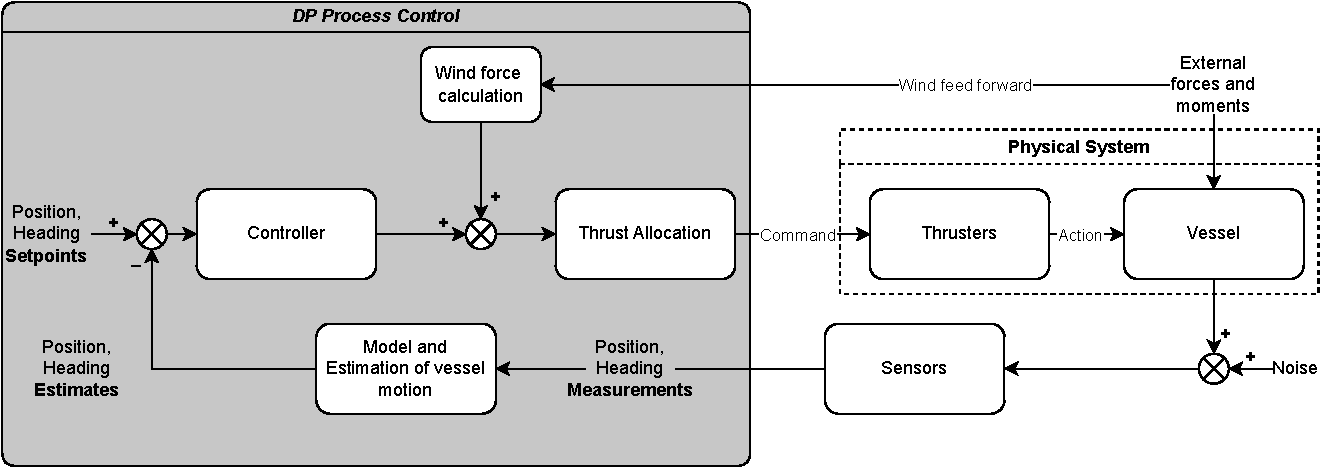
\includegraphics[width=0.75\linewidth]{report/images/diagrams/DP_overview.pdf}
    \caption{Overview of DP system components}
    \label{fig:dp_overview}
\end{figure}




\chapter{Uncertainty Quantification}



This chapter will investigate the fundamentals of uncertainty quantification. Techniques and methods relevant to the
prediction of DP performance will be identified and documented.

\section{What is Uncertainty Quantification?}
A typical uncertainty quantification problem involves a mathematical model, subject to
uncertainty about the correct parameter values \parencite{sullivanIntroductionUncertaintyQuantification2015}.
\textcite{higdonUncertaintyQuantificationError2009} define uncertainty quantification as follows:

\begin{quotation}
    "Uncertainty quantification (UQ) studies all sources of error and uncertainty, including the following: systematic
    and stochastic measurement error; ignorance; limitations of theoretical models; limitations of numerical
    representations of those models; limitations of the accuracy and reliability of computations, approximations, and
    algorithms; and human error. A more precise definition is UQ is the end-to-end study of the reliability of
    scientific inferences"
    \parencite{higdonUncertaintyQuantificationError2009}.
\end{quotation}

In general in the study of UQ, one is interested in the relationship between the input and output. Two general examples
are the forward and the inverse problem \parencite{sullivanIntroductionUncertaintyQuantification2015}. In both examples
we will consider a general model of a physical system:
\[
z = f(x, y)
\]

In the forward problem, $f, \, x, \, y$ are known. $z$ can be calculated. However, if $f$ is an imperfect model or $x,
\, y$ are subject to some uncertainty, then this uncertainty will in some way affect $z$. This is known as the 
\textit{forward propegation of uncertainty}.

In the inverse problem $z, \, x,\, y$ are measured. We are interested in determining $f$. These measurements are subject to noise and as $f$ is a model of a
real system and thus has infinitely many degrees of freedom, the problem is undetermined. 


\section{Sensitivity analysis}
In this section sensitivity analysis will be discussed. Sensitivity analysis is the understanding of how a function
$f(x_1, \dots, x_n)$ depends on variations in $x_i$, both individually and in combinanation with other $x_i$
\parencite{sullivanIntroductionUncertaintyQuantification2015}. There are two approaches: local sensitivity analysis and
global sensitivity analysis. Local analyses study how the system responds to input variations around a point
$\overbar{x}$. Global sensitivity analyes study the average sensitivity of $f$ to variations across the entire domain. A
practical application is that understanding the sensitivity of a system can allow an engineer to decide which variables
to include uncertainty of in their uncertainty modelling. 

\section{Intrusive Methods}
Intrusive methods for uncertainty quantification are methods that require alteration of the governing equations ot
incorporate uncertainty directly.

\section{Polynomical Chaos Expansions}
Polynomial chaos expansions (PCE) are a spectral method for uncertainty quantification. A spectral mathod is a method where a
stochastic process is represented as a series expansion using an orthogonal basis of functions. Spectral methods
decompose a random variable into components, similar to a fourier analysis \parencite{heuvelineHybridGeneralizedPolynomial2014}.

PCE uses polynomials as the orthogonal basis

\section{Non-intrusive methods}
Non-intrusive methods for uncertainty quantification are methods that allow the use of existing models as a black box
without adjusting their internal structure for UQ. 

\textcite{sullivanIntroductionUncertaintyQuantification2015} discusses several of these methods. The guiding principle
of these is that the function is evaluated at a number of points. A surrogate model is then made based on these samples.
The first method discussed is a non-intrusive spectral projection. With this method the aim is to select the best
polynomial chaos coefficients so as to model the function best using a set of orthogonal polynomials.
The second method, stochastic collocation, creates an interpolant between chosen nodes. The third method is gaussian
process regression. This method, in contrast to the two previous methods, does not assume perfectly accurate
observations. The function is assumed to be a random gaussian field and any observations made reduce the uncertainty at
those points.

One important aspect to note is that these methods all assume the function does not change in time. This makes these
methods as is unsuitable for dynamic systems. 


\chapter{Surrogate Modelling}

\section{NARX}
Nonlinear Autoregressive with exogeneous input models 

\section{Neural Networks}

\subsection{DeepAR}

\subsection{LSTM}

\subsection{XGBoost with Quantile Regression}

%% Use letters for the chapter numbers of the appendices.
% \appendix

% \input{a_example}

\printbibliography


\end{document}

